\section{Method}
Time has not yet allowed for the creation of a neat and detailed test plan. However, before the voltage regulator boards are soldered onto the main board, they need to be thoroughly tested to verify their functionality. The plan is to create a test table for this purpose, similar to the specification of ICs in datasheets.

\subsection{Hardware}
\subsubsection{Buck}
Due to the limited time, this verification has not been done yet.

\subsubsection{SEPIC}
For the xxxx, the following parameters need to be measured to demonstrate proper operation:
-Thorough visual inspection, especially focusing on the soldering process. This includes checking for short circuits, open connections, solder balls, and other defects.
-The converter should be powered from a lab power supply with low current limit settings. In case of a short circuit or other module defect, the dissipated power will be limited, allowing for the identification and resolution of the issue.
-The output voltage of the converter should be observed using an oscilloscope. Attention should be paid to the absolute accuracy and the amplitude of the ripple voltage.
-The temperature of the PCBA should be monitored to ensure that the module does not get too hot, which could potentially shorten its lifespan.

\subsubsection{Linear voltage regulator}
After conducting a thorough visual inspection, it became apparent that a thorough cleaning of the PCBA was necessary. This was because the solder paste used left behind a significant amount of residue. Therefore, the linear voltage regulators were cleaned in an ultrasonic cleaner.

Subsequently, the linear regulators were connected to a lab power supply with current limiting. However, it quickly became evident that the regulators were not functioning properly. After performing several simulations in LTspice, it was suspected that the LEDs, which serve as low-noise voltage references, might have been soldered incorrectly. However, after consulting the datasheet again with several group members, it was confirmed that the LEDs were indeed soldered correctly according to the datasheet.

Since no other plausible causes emerged after further investigation, it was decided to desolder one of the LEDs and measure it out of circuit using a multimeter to determine its polarity and threshold voltage. To the astonishment of the group, it was discovered that the Broadcom datasheet for the HSMH-C170 LED did not match the LEDs actually supplied. The polarity marking in the datasheet was the exact opposite of the actual component. It is unknown whether an incorrect batch was delivered or if the datasheet itself is genuinely incorrect.
%https://nl.mouser.com/datasheet/2/678/AV02_0551EN_DS_HSMx_Cxxx_25Mar2022-1827675.pdf

\subsubsection{Main board}

\subsection{Firmware}

\section{Results}

\subsection{Hardware}

\subsubsection{Buck}
Due to the limited time, this verification has not been done yet.

\subsubsection{SEPIC}

\ref{Verification_SEPIC_1A_Load}.


\begin{figure}[ht]
    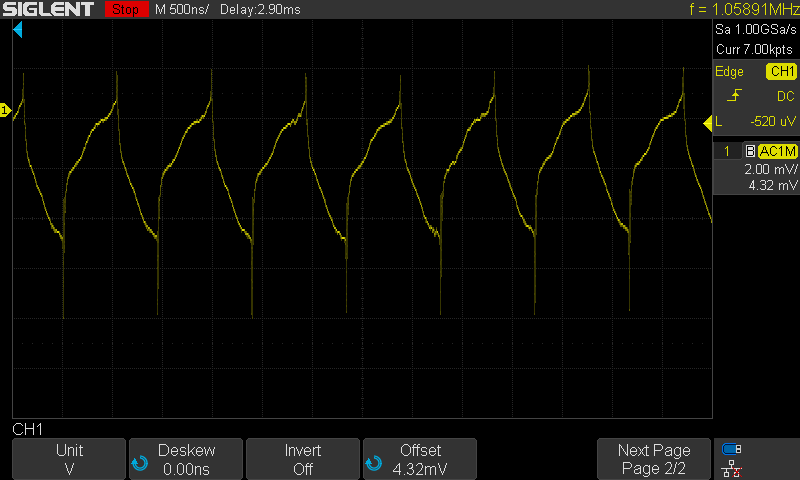
\includegraphics[width=\linewidth]{SEPIC_1A_load.png}
    \caption{SEPIC output voltage at 1A load}
    \label{fig:Verification_SEPIC_1A_Load}
\end{figure}

\section{Conclusions}

\subsection{Hardware}

\subsubsection{Buck}
Due to the limited time, this verification has not been done yet.

\subsubsection{SEPIC}
The SEPIC appears to be functioning well after some quick measurements. With an input voltage of +12V, it generates a stable -15V output voltage, and the voltage ripple remains nearly constant regardless of the output current. This aligns with the calculations and simulations. Additionally, the amplitude of the output ripple voltage closely matches the calculated and simulated values.

\subsubsection{Linear voltage regulator}
Due to the limited time, this verification has not been done yet.

\subsubsection{Main board}
Due to the limited time, this verification has not been done yet.

\subsection{Firmware}